\chapter{How to Speak with Meaning}

This lecture begins with a deceptively simple observation: the choice between memorizing a script, reading from it, or speaking from notes is not yet the heart of the matter. The real question is what live delivery adds to words that already exist on the page. The answer unfolds in a deliberate sequence. First, a talk acquires force by adding a human layer to information. Second, that layer must be organized through two variables we can actually work on, voice and body. The lecture is therefore practical from the beginning: it asks what changes in the listener, what changes in the speaker, and how we can make those changes on purpose.

\section{Why Not Just Email the Script?}

The opening move is not a technique but a challenge. If the words are already available in written form, why not simply send them to the audience and spare everyone the trouble of performance? This question matters because it strips away the comforting illusion that delivery is decorative. If the spoken version contributes nothing essential, then the talk itself is unnecessary.

The lecture answers this by insisting that a talk is not merely a transport mechanism for sentences. A written page can deliver information, but a living voice and a living body can also shape attention, trust, emphasis, and urgency. In that sense, the first contrast in the lecture is already structural:
\begin{equation}
\text{printed words alone} \neq \text{live talk with human layer}.
\end{equation}

\subsection{Question \& Answer}

\paragraph{Question.} If the words are already written, why give a talk instead of sending the text?

\paragraph{Answer.} Because the live talk is not redundant with the text. The spoken event changes how the audience receives the words. It does not merely move information from one place to another; it adds a layer of human force that a page by itself cannot supply.

A useful way to picture the lecturer's question is as a communication geometry: one center, many listeners.
\begin{equation}
\text{speaker/message} \longrightarrow \text{audience members}.
\end{equation}

\begin{figure}[h]
\centering

\includegraphics[width=0.58\textwidth]{how_to_speak_with_meaning_figure_02.png}
\end{figure}

\begin{figure}[h]
\centering
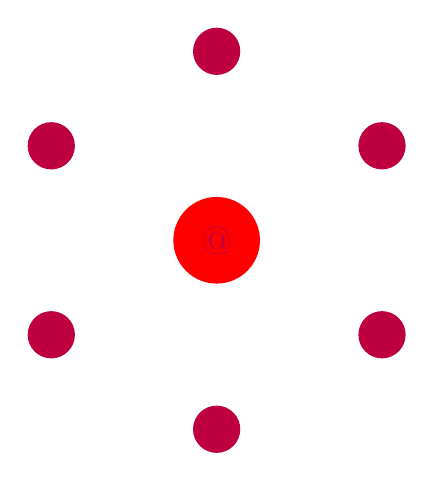
\begin{tikzpicture}[scale=1.0]
\fill[red] (0,0) circle (0.55);
\node[color=purple] at (0,0) {\Large @};

\fill[purple] (0,2.4) circle (0.30);
\fill[purple] (2.1,1.2) circle (0.30);
\fill[purple] (2.1,-1.2) circle (0.30);
\fill[purple] (0,-2.4) circle (0.30);
\fill[purple] (-2.1,-1.2) circle (0.30);
\fill[purple] (-2.1,1.2) circle (0.30);
\end{tikzpicture}
\end{figure}

The slide itself is deliberately spare. It does not try to prove anything. It simply isolates the problem: if a message can be centered and distributed, why is the performance needed? The lecture keeps that question alive long enough to force a serious answer.

\section{Humanity and Inspiration}

The answer comes in two stages. First, the lecturer names the missing ingredient: our humanity. Second, he shows what that ingredient does. A human presence can make an audience say, ``I trust this person,'' or ``Now I understand why that word mattered,'' or ``I can hear the excitement, the hurt, the conviction.'' The lecture is careful here: it does not define humanity in abstraction, but through its effects on a listener.

Those effects accumulate. Trust, heightened interest, heard emphasis, empathy, excitement, conviction, and willingness to act are not separate ornaments. They are successive ways in which information is made active in another mind. The lecture compresses that whole chain into a single word: inspiration.

\subsection{Question \& Answer}

\paragraph{Question.} What is the ``something extra'' that a live talk adds beyond the script?

\paragraph{Answer.} The extra term is the speaker's humanity, not as a vague virtue, but as a set of audible and visible signals that alter reception. Humanity turns information into something the audience can feel, trust, and act on.

We can summarize the lecturer's claim schematically:
\begin{equation}
\text{humanity} + \text{information} \Longrightarrow \text{inspiration}.
\end{equation}

\begin{definition}
In this lecture, \emph{inspiration} is not a mystical quality. It is the force that tells the mind what to do with a new idea rather than letting that idea be filed away and forgotten.
\end{definition}

This gives us a useful contrast:
\begin{align}
\text{ordinary idea} &\Longrightarrow \text{filed away}, \\
\text{inspiration} &\Longrightarrow \text{attention alert}.
\end{align}

The lecture's order is important. We are not first given a list of speaking techniques and then told what they are for. We are first shown the goal on the listener's side. Only after that does the lecture ask what the speaker can control.

\section{Two Variables: Voice and Body}

Once inspiration has been defined functionally, the lecture pivots from outcome to method. If we want a talk to carry that human force, what are the main variables we can actually work on? The lecturer answers with a clean decomposition: voice and body.

\subsection{Question \& Answer}

\paragraph{Question.} What are the two major things we should optimize when preparing a talk?

\paragraph{Answer.} We should ask two questions. What are we doing with the voice? And what are we doing with the body? Everything that follows in the lecture is organized around that split.

The decomposition can be written compactly as
\begin{equation}
\text{talk preparation} \Longrightarrow \text{voice} + \text{body}.
\end{equation}

The corresponding slide records this as a branching structure. Visually it is a question that leads into a choice structure with contrasting outcomes. The transcript then resolves the abstraction by naming the two branches explicitly in prose.

\begin{figure}[h]
\centering

\includegraphics[width=0.68\textwidth]{how_to_speak_with_meaning_figure_03.png}
\end{figure}

\begin{figure}[h]
\centering
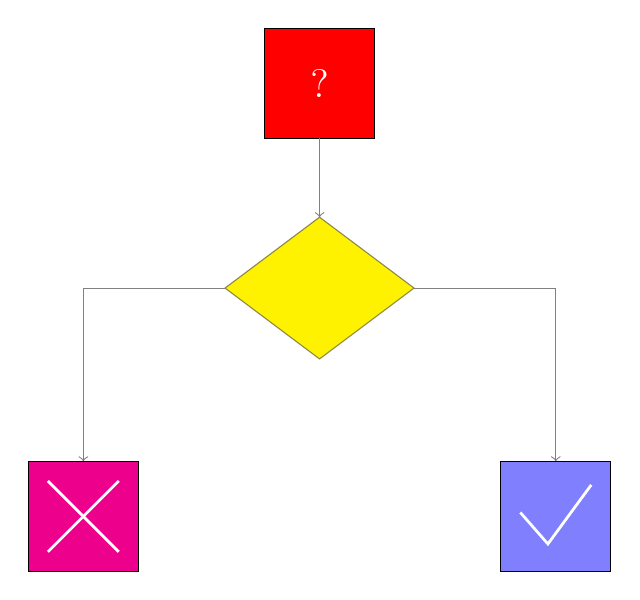
\begin{tikzpicture}[scale=1.0]
\draw[fill=red] (-0.7,2.4) rectangle (0.7,3.8);
\node[color=white] at (0,3.1) {\Large ?};

\draw[->, gray] (0,2.4) -- (0,1.4);

\draw[fill=yellow, draw=yellow!50!black] (0,1.4) -- (-1.2,0.5) -- (0,-0.4) -- (1.2,0.5) -- cycle;

\draw[gray] (-1.2,0.5) -- (-3.0,0.5) -- (-3.0,-1.0);
\draw[gray] (1.2,0.5) -- (3.0,0.5) -- (3.0,-1.0);
\draw[->, gray] (-3.0,-1.0) -- (-3.0,-1.7);
\draw[->, gray] (3.0,-1.0) -- (3.0,-1.7);

\draw[fill=magenta] (-3.7,-3.1) rectangle (-2.3,-1.7);
\draw[white, line width=1pt] (-3.45,-2.85) -- (-2.55,-1.95);
\draw[white, line width=1pt] (-3.45,-1.95) -- (-2.55,-2.85);

\draw[fill=blue!50] (2.3,-3.1) rectangle (3.7,-1.7);
\draw[white, line width=1pt] (2.55,-2.35) -- (2.9,-2.75) -- (3.45,-2.0);
\end{tikzpicture}
\end{figure}

The picture itself is more abstract than the transcript. It gives us the structure of division; the lecture then fills that structure with content. That is a pattern worth preserving in the notes: first a large question, then a clean split, then a detailed treatment of each term.

\section{Voice: Variety That Follows Meaning}

The lecture enters the first branch, voice, by example rather than by theory. We are asked to listen to the opening minute of George Monbiot and to notice the effect before we are told the mechanism. The exact details of the anecdote matter less here than the speaker's control: his voice does not sit on the surface of the words. It enters them and gives them contour.

That is why the audience feels pulled into his world. The words may be interesting on the page, but the talk becomes compelling because the delivery distinguishes among them. Some phrases expand, some contract, some slow down, some turn, some land. We hear hierarchy.

\subsection{Question \& Answer}

\paragraph{Question.} How does a speaker make words feel alive rather than merely correct?

\paragraph{Answer.} By creating variety in the voice that is governed by meaning. The point is not random expressiveness. The point is that the sound of the sentence changes when the meaning changes.

The lecture's rule may be written as
\begin{equation}
\text{variety in speech} \Longrightarrow \text{meaning made audible}.
\end{equation}

The negative example is equally important. A monotone delivery is not merely dull. It carries a false mathematical signal: it tells the audience that no local region of the talk has more weight than any other. The lecture therefore diagnoses monotony structurally:
\begin{equation}
\text{every sentence sounds the same} \Longrightarrow \text{no part seems more important than any other}.
\end{equation}

The lecturer gives a few characteristic symptoms of this failure mode: a small rise at the start of each sentence, a drop at the end, no pauses, and no change of pace. The result is a uniform field. Once the voice becomes uniform, the argument becomes flat, and the audience drifts.

\section{Marking the Script So the Voice Can Move}

The lecture now becomes algorithmic. If a talk is scripted, we are told not to hope that variation will appear by accident. We should write the structure of emphasis onto the page itself. That advice is more rigorous than it first sounds. It amounts to constructing a visible map from textual structure to vocal behavior.

\subsection{Question \& Answer}

\paragraph{Question.} How can a scripted talk be marked so that the voice varies with meaning instead of slipping into monotone?

\paragraph{Answer.} We mark the script in layers. First we underline the important words in each sentence. Then we identify the one governing word in each paragraph and underline it twice. After that we add special marks for special local tasks: questions, playful passages, jokes, and the main aha moment.

The governing notation may be written as
\begin{align}
\underline{\text{important word}}, \qquad
\underline{\underline{\text{paragraph key word}}}.
\end{align}

The slide does not show literal text. It shows the structure of the procedure: paragraph-like lines with selected underlines. The abstraction is useful because it tells us that this is not about a particular script, but about a general method of annotation.

\begin{figure}[h]
\centering

\includegraphics[width=0.63\textwidth]{how_to_speak_with_meaning_figure_04.png}
\end{figure}

\begin{figure}[h]
\centering
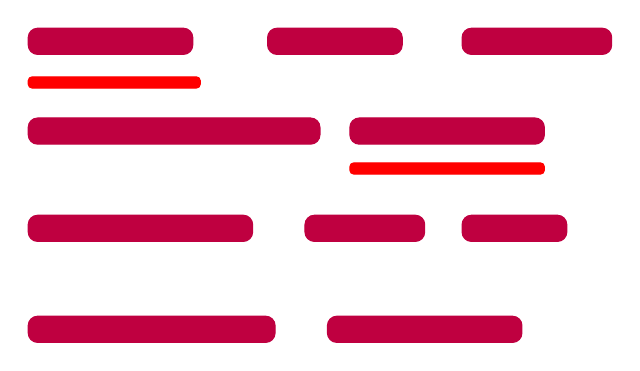
\begin{tikzpicture}[scale=0.95]
\draw[fill=purple, draw=purple, rounded corners=0.12cm] (-3.1,2.4) rectangle (-0.9,2.75);
\draw[fill=purple, draw=purple, rounded corners=0.12cm] (0.1,2.4) rectangle (1.9,2.75);
\draw[fill=purple, draw=purple, rounded corners=0.12cm] (2.7,2.4) rectangle (4.7,2.75);

\draw[fill=red, draw=red, rounded corners=0.05cm] (-3.1,1.95) rectangle (-0.8,2.1);

\draw[fill=purple, draw=purple, rounded corners=0.12cm] (-3.1,1.2) rectangle (0.8,1.55);
\draw[fill=purple, draw=purple, rounded corners=0.12cm] (1.2,1.2) rectangle (3.8,1.55);

\draw[fill=red, draw=red, rounded corners=0.05cm] (1.2,0.8) rectangle (3.8,0.95);

\draw[fill=purple, draw=purple, rounded corners=0.12cm] (-3.1,-0.1) rectangle (-0.1,0.25);
\draw[fill=purple, draw=purple, rounded corners=0.12cm] (0.6,-0.1) rectangle (2.2,0.25);
\draw[fill=purple, draw=purple, rounded corners=0.12cm] (2.7,-0.1) rectangle (4.1,0.25);

\draw[fill=purple, draw=purple, rounded corners=0.12cm] (-3.1,-1.45) rectangle (0.2,-1.1);
\draw[fill=purple, draw=purple, rounded corners=0.12cm] (0.9,-1.45) rectangle (3.5,-1.1);
\end{tikzpicture}
\end{figure}

The lecture also gives a second family of marks:
\begin{align}
\text{question mark} &\mapsto \text{highlight}, \\
\text{playful passage} &\mapsto \text{wavy underline}, \\
\text{aha moment} &\mapsto \text{black blob before it}, \\
\text{joke} &\mapsto \text{pink dots above it}.
\end{align}

From these marks comes the operational rule
\begin{equation}
\text{script marks} \Longrightarrow \text{corresponding vocal changes}.
\end{equation}

\paragraph{Worked procedure.} The lecture's algorithm can be written as a short derivation from page structure to delivery structure.
\begin{enumerate}
\item Begin with the written script and scan sentence by sentence.
\item In each sentence, select the two or three words that carry the local load and underline them.
\item In each paragraph, identify the one word that governs the paragraph's movement and underline it twice.
\item Add special symbols for questions, playfulness, humor, and the main aha moment.
\item Read the script again, but now let pace, pause, loudness, and softness respond to those marks.
\item Repeat once more, this time letting the emotion attached to each section enter the voice.
\end{enumerate}

This last step matters. The lecture is careful not to let the method become mechanical. After the marks are in place, we are told to remember the emotions associated with each section --- passion, anger, laughter, confusion --- and to let those emotions out a little in the read-through. The check on the whole process is empirical: try it with a friend, or record it and listen back with closed eyes.

\section{Body: Stance, Movement, and Stillness}

The second half of the lecture begins from another failure mode. A speaker may come onstage looking as though the body is merely a device for transporting the head. Once there, the body becomes uncertain: hands fixed at the sides, weight shifting, feet rocking, motion without intention. The lecture does not attack this morally. It treats it as a problem of control and legibility.

The first correction is extremely simple: stand tall, and distribute weight evenly. That is a bodily analogue of balance in an equation. The point is not stiffness. The point is stability.

\subsection{Question \& Answer}

\paragraph{Question.} Should a speaker stand still or move around the stage?

\paragraph{Answer.} Either can work. But movement must have purpose, and stillness must be available. The audience should see a controlled rhythm, not a leak of nervous energy.

The balance condition is expressed visually by the slide and may be written in cleaned form as
\begin{equation}
\text{weight on left foot} = \text{weight on right foot}.
\end{equation}

\begin{figure}[h]
\centering

\includegraphics[width=0.56\textwidth]{how_to_speak_with_meaning_figure_05.png}
\end{figure}

This is a cautious reconstruction: the equals sign is visible, while the spoken instruction supplies the interpreted variables. The lecture then broadens the prescription. Once the stance is stable, the upper body may move freely. The hands and arms may emphasize what is being said. Good posture helps. Slouching should be avoided.

But the lecture does not stop at stillness. Some speakers prefer to walk the stage, and walking can work. What matters is the rhythm:
\begin{equation}
\text{purposeful movement} + \text{moments of stillness} \Longrightarrow \text{powerful stage rhythm}.
\end{equation}

The corresponding warning is just as clear:
\begin{equation}
\text{constant pacing or rocking} \Longrightarrow \text{visible discomfort for the audience}.
\end{equation}

\paragraph{Practical rule.} We may write the bodily advice as a short control law.
\begin{enumerate}
\item Establish a stable base.
\item Let gesture arise naturally from the content.
\item Move only when movement helps thought or emphasis.
\item Stop moving when an important point must land.
\item Eliminate repetitive rocking, because it advertises anxiety rather than meaning.
\end{enumerate}

The lecture ends this section by refusing to turn the advice into dogma. Some speakers sit. Some walk. Some move with great energy. The standard is not uniform style. The standard is whether the body supports the message without distracting from it. That is why the final test remains rehearsal: show it to a small audience, or watch yourself back, and ask whether the body is helping the idea travel cleanly.

\section{Summary}

The lecture's logic is compact once we see its shape. A talk matters because live delivery adds something a page cannot: a human layer. That layer changes reception and turns information into inspiration. To build that effect deliberately, we decompose preparation into two variables, voice and body.

On the side of voice, the main principle is that variation must follow meaning. Monotony is not only dull; it falsely levels the argument. The practical remedy is to mark the script and let those marks govern pace, pause, softness, emphasis, and emotional color. On the side of body, the main principle is calm power. We begin with balance, allow natural gesture, use movement only with purpose, and preserve stillness for important points.

The lecture therefore ends where it must. There is no single presentation style to imitate. What we want is a way of speaking and standing that lets the idea come through with force, clarity, and unmistakable human presence.